\documentclass{vldb}

\newcommand{\paperTitle}{Efficient Content-Based Audio Retrieval}
\newcommand{\paperKeywords}{Audio Retrieval, Deep Learning}
\newcommand{\paperAuthors}{}

\vldbTitle{\paperTitle}
\vldbAuthors{\paperAuthors}
\vldbDOI{https://doi.org/10.14778/xxxxxxx.xxxxxxx}
\vldbVolume{xx}
\vldbNumber{yyy}
\vldbYear{2019}

\setlength{\paperheight}{11in}
\setlength{\paperwidth}{8.5in}

%\usepackage[square,numbers]{natbib}
\usepackage[hyphens]{url}
\usepackage{xstring}

\usepackage[usenames,dvipsnames]{xcolor}
\definecolor{linkcolor}{HTML}{647382}
\definecolor{citecolor}{HTML}{647382} %
\definecolor{urlcolor}{rgb}{0.4,0.2,0.2}
\definecolor{sqlcolor}{HTML}{965d67}
\definecolor{smtcolor}{HTML}{5d968c}

\usepackage[breaklinks]{hyperref}
\hypersetup{%
    pdfauthor = {\paperAuthors},
    pdftitle = {\paperTitle},
    pdfkeywords = {\paperKeywords},
    bookmarksopen = {true},
    colorlinks=true,
    citecolor={urlcolor},
    linkcolor={linkcolor},
 	urlcolor={citecolor},
    pdfborder={ 0 0 0 }
}

\usepackage[usenames,dvipsnames]{xcolor}
\usepackage{amsmath,amsopn,amssymb}
\DeclareMathOperator*{\argmax}{arg\,max}
\DeclareMathOperator*{\argmin}{arg\,min}

\usepackage{listings}
\usepackage[caption=false]{subfig}
\usepackage{endnotes,microtype,xspace,graphicx,fancyvrb,multirow}
\usepackage{supertabular,booktabs}
\usepackage{array,underscore,relsize}
\usepackage[T1]{fontenc}
\usepackage{times}
\usepackage{fancyhdr,lastpage}
\usepackage{enumitem}
\usepackage{balance}
\usepackage{booktabs}
\usepackage{pifont}
\usepackage{listings}
\usepackage{multirow}
\usepackage[scaled]{beramono}
\usepackage{tabularx}
\usepackage{wrapfig}

% stmaryrd: more math fonts (namely mathbb)
\usepackage{stmaryrd}
\usepackage{ltablex}
\usepackage{mathtools}

% algorithm2e: algorithms
\usepackage{amsmath}
\usepackage[ruled,linesnumbered]{algorithm2e}
\usepackage{enumitem}
\usepackage{algpseudocode}

\SetAlFnt{\small}
\SetAlCapFnt{\small}
\SetAlCapNameFnt{\small}

\def\Snospace~{\S{}}
\renewcommand*\sectionautorefname{\Snospace}
\def\sectionautorefname{\Snospace}
\def\subsectionautorefname{\Snospace}
\def\subsubsectionautorefname{\Snospace}
\def\chapterautorefname{\Snospace}


% cleveref goes last to get alg name right
\usepackage[capitalize,noabbrev]{cleveref}

\widowpenalty10000
\clubpenalty10000

% captions
\captionsetup{font=small}
\captionsetup{labelfont=bf}
\captionsetup[subfloat]{font=scriptsize}
\captionsetup[subfloat]{farskip=5pt}
\captionsetup[subfloat]{captionskip=1pt}
\captionsetup[table]{belowskip=0pt}

\captionsetup[table]{position=t}
\captionsetup[table]{skip=\medskipamount}

\setlength{\textfloatsep}{0.1cm}

% captions placed on the bottom for figures
\captionsetup[figure]{position=b}
%figures and tables numbered by section
%\captionsetup{figurewithin=section}
%\captionsetup{tablewithin=section}

% % Squished Lists
\newcommand{\squishitemize}{
 \begin{list}{$\bullet$}
  { \setlength{\itemsep}{0pt}
     \setlength{\parsep}{3pt}
     \setlength{\topsep}{3pt}
     \setlength{\partopsep}{0pt}
     \setlength{\leftmargin}{1.95em}
     \setlength{\labelwidth}{1.5em}
     \setlength{\labelsep}{0.5em} } }

\newcounter{Lcount}
\newcommand{\squishlist}{
    \begin{list}{\arabic{Lcount}. }
   { \usecounter{Lcount}
        \setlength{\itemsep}{0pt}
        \setlength{\parsep}{3pt}
        \setlength{\topsep}{3pt}
        \setlength{\partopsep}{0pt}
        \setlength{\leftmargin}{2em}
        \setlength{\labelwidth}{1.5em}
        \setlength{\labelsep}{0.5em} } }

\newcommand{\squishend}{\end{list}}

\newcommand{\eg}{e.g.}
\newcommand{\ie}{i.e.}

\newcommand{\PP}[1]{
%\vspace{4px}
\noindent{\bf{#1}.}\xspace
}

% per-author notes:
% ref. http://en.wikibooks.org/wiki/LaTeX/Colors
\newcommand{\PJ}[1]{\textcolor{Blue}{PJ: #1}}
\newcommand{\AJ}[1]{\textcolor{Red}{AJ: #1}}

%% ==================================================================
%% MAGIC FIGURE SPACING
%% ==================================================================

% Single-Column Figures
\setlength{\floatsep}{5pt}
% \setlength{\textfloatsep}{5pt}
\setlength{\abovecaptionskip}{0.5em}
\setlength{\belowcaptionskip}{0.5em}

%% Multi-Column Figures
\setlength{\dbltextfloatsep}{5pt}
\setlength{\dblfloatsep}{5pt}

% Subfigures
% \setlength{\subfigcapskip}{0in}
% \setlength{\subfigtopskip}{0pt}
% \setlength{\subfigbottomskip}{2pt}

\pagestyle{fancy}
\fancyhf{}
\renewcommand{\headrulewidth}{0pt}
\cfoot{\thepage}

\newcommand{\sys}{\mbox{\textsc{Echo}}\xspace}

\newcommand*{\refname}{Bibliography}

\graphicspath{ {./figures/} }

\title{\paperTitle\vspace*{-0.15in}}
\author{\paperAuthors}

\begin{document}

\newcommand{\mail}[1]{\href{mailto:#1}{#1}}

\title{\paperTitle}

\author{ \def\arraystretch{1}
\begin{tabular}{ cc }
Jacob Logas  & Joy Arulraj \\
\multicolumn{1}{c}{\mail{logasja@gatech.edu}} &
\multicolumn{1}{c}{\mail{arulraj@gatech.edu}} \\
\end{tabular}
}

\maketitle

\begin{abstract}
The integration of microphones in smartphones and wearables has led to 
an increase in the volume of human-generated audio recordings.
Similarly, the advent of autonomous wireless recording devices has led to 
an increase in the volume of animal-generated audio recordings.
Given the shrinking cost of data storage, it is now easy and inexpensive 
to capture and store a large database of audio recordings.
The information recorded in such a database would be invaluable if an user 
can efficiently search the contents of the database.

Researchers have designed audio data management systems for automatically
finding recordings that are relevant to an user's search query.
However, the state-of-the-art approach for automated content-based audio
retrieval suffers from two limitations.
First, its application of image-centric retrieval techniques to audio
spectrograms limits accuracy, thereby restricting the efficacy of 
searching the database.
Second, it employs a computationally-expensive classical machine learning 
model that restricts the efficiency of search pipeline.

This paper makes the case for an alternate approach for content-based audio
retrieval using text queries.
The key idea is to use domain knowledge of the structure of audio and 
human perception to retrieve relevant recordings with high probability.
We have implemented our audio-centric representation, classification, and
retrieval techniques in \sys.
Our evaluation shows that \sys is 5$\times$ faster than the state-of-the-art 
system by virtue of being designed for audio recordings instead of images.
We anticipate that \sys will allow an user to effectively and efficiently 
explore large unstructured audio datasets.
\end{abstract}

\section{Introduction}

The audible world holds much information, often information that we as humans
either cannot hear or ignore in favor for other sensory cues. Through audio
alone, machine learning (ML) models have been able to accurately determine 
the inner state of an animal or a human or even an environment, 
a task which is often accomplished through visual cues~\cite{Farago2010,
schuller-acoustic-2009,Eronen2006}. 

Over the last decade, audio has become easier to collect in environments ranging
from in-home microphones in intelligent assistants to wireless recording 
wearables in an ocean setting~\cite{kohlsdorf-underwater-2013,Lane2015,
Choudhury2008}.
This is in part a consequence of embedded systems becoming smaller and more
efficient as well as improvements in the quality of miniature
microphones\AJ{Cite}.
This increase of audio sources has led to an increase in the volume of audio
recordings. Given the shrinking cost of data storage, it is now easy and
inexpensive to capture and store a large database of recordings.
The information recorded in such a database would be invaluable if an user 
can efficiently search the contents of the database.

%In human speech, speaker discrimination is also possible
%and has found its way into several intelligent assistants \cite{Campbell1997}.
%Finally, perhaps the best known and most widely studied application for audio
% is obtaining textual representations of speech \cite{Rabiner1989}. These
%applications are unlikely the limit of what we can glean from audio data and
%with audio recording devices becoming more ubiquitous and cheaper than imagery
%collection, we are obtaining more audio from a wider variety of places.

A na\"ive technique for content-based audio retrieval (CBAR) consists of
manually labeling each recording. 
The limitations of this technique are twofold.
First, the number of man-hours required for labeling increases along with the
size of the database.
Second, a manual labeling process can be error-prone resulting in data
being mislabeled or entirely overlooked~\cite{Bardeli2009,Rong2018}. 

A more scalable technique requires the user to only label a subset of the
database.
With this CBAR technique, the user is presented with statistically significant
examples that they may have previously missed\AJ{Cite}.
The audio database management system (DBMS) uses exemplars of the 
user-specified recording to find other similar recordings in the database
using a \textit{similarity search} algorithm.
This technique is restrictive in two ways.
First, it requires an exemplar of all desired audio segments which may defeat
the purpose of searching the database and does not support exploratory data
analysis. 
Second, the DBMS must check the similarity of every recording in the database.
The recent surge in the volume of generated audio data has led to an increase 
in the size of audio databases. This technique does not scale to such 
databases due to the computational cost of the similarity search algorithm.

To address these limitations of traditional CBAR techniques, researchers have
proposed an alternate ML model that leverages a compact data
representation~\cite{Chechik2008}. This technique consists of transforming
audio recordings to images via spectroscopy and then applying the ML for
retrieving relevant images. \AJ{Perf comparsion to previous techniques}.
However, applying image-centric retrieval techniques to audio spectrograms
limits the accuracy and efficiency of the audio DBMS.
We attribute this to the \textit{transparency} of audio data. 
Unlike images, audio recordings are often derived from a collection of audio
sources that can overlap in their frequency ranges.

A better approach is to use audio-aware data representation and retrieval
algorithms. This paper investigates the efficacy and efficiency of an ML 
model that is guided by a taxonomy of human audio perception~\cite{Gaver1993}.
We formulate a hierarchical data representation based on low-level intensity,
spectral, and statistical properties that define a given recording. 
%This representation transforms these temporal properties to high-level 
%cognitive properties.
Perception is of interest as the human cognitive capacity continues to exceed
that of machines. Prior work in psychology and physiology has studied 
how and why human perception is accurate and how it can optimally encode audio
~\cite{Gaver1993, Eggermont2001, slaney1993importance, Piazza2013}.
We hypothesize that a more performant and accurate CBAR technique can be
constructed by modeling human auditory systems.
We implemented our audio-centric representation, classification, and retrieval
techniques in \sys. We validated our hypothesis by comparing \sys against 
the state-of-the-art CBAR technique.

In all, the contributions this work provides is as follows:
\begin{itemize}
    \item Present an audio representation based on human perception of sound.
    \item Demonstrate a model developed to match the Gaver taxonomy of sound.
    \item Use probabilistic models to retrieve unstructured data with high confidence.
\end{itemize}
\section{Motivation}
%\begin{itemize}
%    \item Machine Hearing Principles
%    \item Spectrogram Based Machine Hearing
%    \item Case for Audio-Based Machine Hearing (w/ results teaser)
%\end{itemize}

We begin with an overview of machine hearing principles and make the case for 
an audio-centric CBAR technique.

\subsection{Machine Hearing Principles}
\label{motivation:machine-hearing}

Machine hearing is an emerging field focused on endowing machines with  
the ability to hear as humans do~\cite{lyon-human-2017}.
%However, this field has lagged behind computer vision due to its seeming lack
% of general applicability. 
%This is shown by the wealth of specialized music and
%speech sound analyses, with more general problems being ignored. 
The goal is to formulate a generalized model of sound with associated
representation, classification, and retrieval techniques. 
The architecture of an audio DBMS for machine hearning, that is inspired by the
human auditory system, consists of three components~\cite{lyon-machine-2010}:

\PP{Representation}
The first component, peripheral analyzer, is based on a part of the inner ear,
called \textit{cochlea} \footnote{Outer-ear structures are at the mercy of the
recording medium (\eg, the microphone).}. 
This spiral-shaped cavity is responsible for forming a representation of the 
given audio data.
by transforming acoustics into neural signals.
\textit{Reissner's membrane} is an important cochlear structure that can be
considered as a collection of band-pass filters, separating sounds into spectral
components~\cite{Plack2018}. These spectral components are then processed by
brain structures that convert the waveform representation to a more compact one.
 
The next step consists of creating an image representation of the given audio
data, thereby modeling the concept of human auditory sensory memory (\ie, echoic
memory) \AJ{Cite}.
The perception of sound depends on what comes before and occurs after an audio
segment. Thus, echoic memory determines human perception. 
It is critical in permitting the listener to integrate incoming information
with past events\footnote{Researchers have not reached consensus on the duration
of the memory  with estimates ranging from 250~ms to four
seconds~\cite{Wingfield2016}.}.
It is challenging to achieve high retrieval accuracy with only the image
representation and as such the next component is used for extracting key
features.

\PP{Classification}
The second component consists of feature extraction module that construct a more
compact and meaningful representation from the image formed by the previous
component.
This module most closely matches the \textit{neural code} of human audio
perception which forms the interface between sound and its conscious perception.
We note that the human auditory processing pipeline is still mostly unknown
and much of what we do know is speculative. 
It is hypothesized that multiple processes occur in
sequence to prepare the information for perception \cite{Eggermont2001}. 
It is likely these processing steps make actual perception less computationally
expensive. The output of this component determines the performance and
efficiency of the final component.

\PP{Retrieval}
This component takes in the representation formed by the previous module 
and maps it decisions. This component is analogous to conscious perception in
humans. It can vary from simple (\eg, a single perceptron) to complex
structures (\eg, a deep neural network).

\subsection{Image-Based Machine Hearing}
% \begin{itemize}
%     \item How this fits into Neural Coding and Echoic Memory
%     \item CNN approach
%     \item Autoencoding CNN approaches
%     \item Image retrieval (PAMIR approach)
% \end{itemize}

Given the high accuracy of content-based image retrieval (CBIR) systems, 
researchers have attempted to leverage these systems for audio retrieval.
Chechik et al. use a passive-aggressive model for image retrieval
(PAMIR) to perform audio retrieval over spectrogram imagery~\cite{Chechik2008}.
This technique consists of transforming audio recordings to spectrograms and
subsequently use image retrieval techniques for audio retrieval.
Thus, it leverages machine vision to perform machine hearing, thereby 
combining the neural coding and echoic memory portions of human hearing 
into a single step \footnote{The vision model is directly trained on
spectrograms instead of relying on a separate classification module.}.

%The PAMIR system uses probabilistic confidence to rank audio recordings based
% on their relevance to a text query.

\begin{figure}[!tbp]
    \centering
    \subfloat[Noisy]{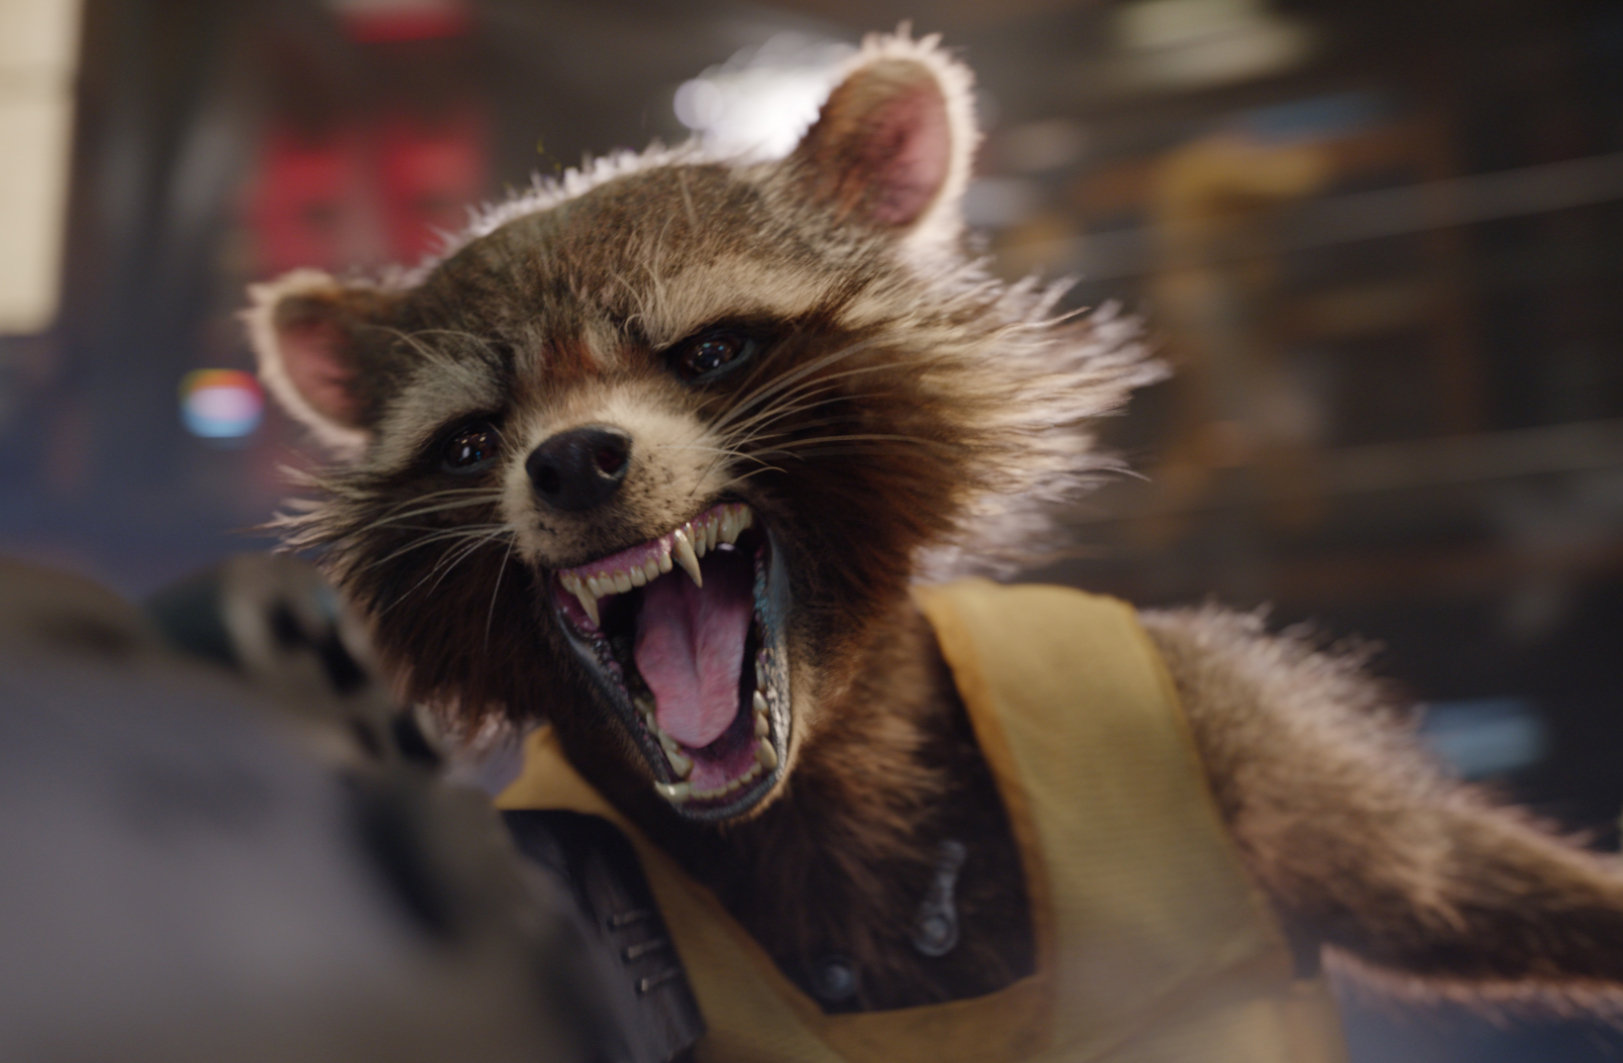
\includegraphics[width=0.5\textwidth]{figures/noisy-audio.jpg}\label{fig:noisy-audio}}
    \hfill
    \subfloat[Clean]{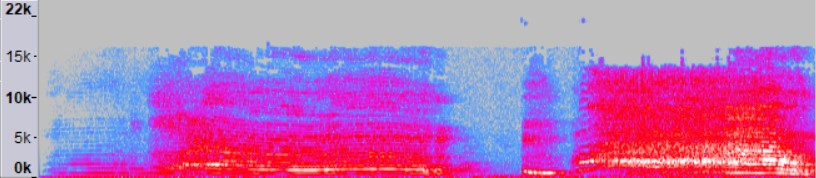
\includegraphics[width=0.5\textwidth]{figures/clean-audio.jpg}\label{fig:clean-audio}}
    \caption{Spectrograms illustrating the difference between clean and noisy audio when converted to the visual domain.}
    \label{fig:noisy-audio-cmpr}
\end{figure}

This approach for translating audio to a visual domain has seen some success,
especially in cases where audio events are isolated as illustrated
in~\cref{fig:noisy-audio-cmpr}.
However, in real-world audio recordings are typically generated from multiple
audio sources often with overlapping frequencies (\eg, group meetings).
This challenge stems from the \textit{transparency} of audio unlike images. 
Thus, a spectrogram is analogous to placing several transparent images 
over one another. 
State-of-the-art CBAR systems use a convolutional neural network (CNN) for 
image classification\AJ{Cite, describe CNN in a few sentences} and
train the CNN model on spectrograms.
However, these systems are unable to deliver high accuracy (> 70\%) even with
complex model ensembles~\cite{xu-large-scale-2018,piczak-environmental-2015}.

A more recent development in image-based machine hearing is to use an
unsupervised learning technique, called \textit{auto-encoding}\AJ{Cite?}. 
An auto-encoder is a type of neural network that learns to reconstruct its 
input image by reducing it to latent variables.
In image-based machine hearing, prior research has focused on reducing 
\textit{spectrogram}\AJ{define?} to latent variables using a CNN.
This approach suffers from the limitations discussed above.
While CNNs are effective on image recognition, they are unable to cope with the
transparency of audio. Furthermore, they ignore key features (\AJ{What?}),
thereby resulting in lower accuracy on real-world audio recordings with
multiple sources.

\subsection{Waveform-Based Machine Hearing}
% \begin{itemize}
%     \item Naive audio features
%     \item DTW + HMM
%     \item Autoencoding RNN approaches
%     \item Biologically Based Encoding
%     \item My approach + some teaser
% \end{itemize}

As an alternative to converting from an audio to visual domain, models can be trained on features from the audio itself. This approach to machine hearing hampers the ability of practitioners to apply proven image-based techniques but is overall more robust. In this approach, models are trained either directly on the audio waveform itself with no transformation, or a spectrogram is calculated and features are extracted from both the waveform and spectrogram.

With waveform-based machine hearing, \textit{Mel-frequency cepstral
coefficients} (MFCCs) are a frequently-used audio representation technique. 
The reasons for their popularity are twofold. First, they computationally
efficient to compute. Next, they provide a representation that is consistent
with human hearing~\cite{kaur-feature-2015}.
While certain audio processing tasks are feasible using only MFCCs, we require 
a more detailed representation for machine hearing\AJ{Cite?}.
A naive solution to this problem is to extract the temporal and spectral
features from the waveform to derive a more complete representation.
However, this approach is computationally expensive and leads to higher data
dimensionality resulting in slower convergence of classification agents.

Other techniques for constructing a detailed representation include: (1) 
Dynamic Time Warping (DTW) and (2) Hidden Markov Models (HMMs).
These approaches directly work on the audio data itself and thus do not require
feature extraction or constructions of spectral images.
They have found success in both speech recognition and specialized retrieval
systems\AJ{Cite?}.
Both DTW and HMMs have the benefit of taking referring back to previous states during determination, thus capturing the sequential nature 
of audio. 
However, DTW is computationally expensive and it is infeasible to support 
large audio databases using this technique.
Similarly, the complexity of HMMs increases when they need to support tens of
classes, as a model must be trained for each class.
Additionally, neither technique takes advantage of domain knowledge 
and do not conform to the machine hearing principles outlined
in~\cref{motivation:machine-hearing}.

While auto-encoding with CNNs does not work well for audio retrieval,
encoders based on Recurrent neural network (RNN) do not suffer from this
limitation.
This is because much of the information in a audio recording is dependent 
on what comes before it.
Unlike CNN-based encoders that learn from the spectrogram image,
RNN-based encoders learn from the waveform values or vectors of spectrogram
features presented as a time series.
The latter approach has two additional benefits.
First, RNN-based encoders are computationally efficient.
Second, they create compact representations that take time into account 
and can be used with any number of off-the-shelf classifiers.

\AJ{Why do we need the following paragraph?}
Researchers continue to seek the biological neural code for audio
encoding~\cite{Eggermont2001}. 
Through studies of the biological systems that convert sound waves to neural
responses, researchers have been able to emulate certain steps of the audio
encoding pipeline with other steps requiring speculation. 
Smith and Lewicki present a non-linear model based on population spike code 
to encode waveforms \cite{smith-efficient-2006}. 
They illustrate that idealized spikes encode precise temporal positions and
magnitudes of underlying acoustic features. 
This effort provides a method to efficiently extract a coding of natural 
sounds, making sure the classifiers are working with an information-rich
representation.

\begin{table}[t]
    \centering
    \begin{tabular}{cccccc}
                & Bag of Features & DTW & HMM & Wavelet  \\ \hline
    Approx Size & a & a & a & a \\
    Complexity  & a & a & a & a
    \end{tabular}
    \caption{Simple table with audio representations and their complexity/usefulness/features}
    \label{tab:audioreps}
\end{table}

We next describe the three components of \sys in detail.

\section{Representation}

In this section, we discuss the representation derived used by \sys to enable
more performant and accurate content-based audio retrieval.
%
~\cref{alg:overall} illustrates the overall flow of the data encoding pipeline.
%
Our goal is to transform the audio waveform into a usable representation for
classification.
%
We next discuss the different stages of the encoding pipeline in detail.

\begin{algorithm}[t!]
    \caption{Construct audio representation for classification.}
	\label{alg:overall}
    \SetKwInOut{Input}{Input}
    \SetKwInOut{Output}{Output}
    \SetKwProg{EncodeAudio}{EncodeAudio}{}{}
    \SetAlgoLined
    
    \EncodeAudio{$(A)$} {
        \Input{Audio recording $A$.}
        \Output{A feature vector $F$ of one or more audio events.}
        $LA \gets LoadAudio(A)$\\
        $TA \gets Tokenize(LA)$\\
        \ForEach{$t_i \in $TA} {
            $F \gets FeatureExtract(t_i)$
        }
        $\Return$ $F$
    }
\end{algorithm}

\subsection{Peripheral Analyzer}
\label{sec:analyzer}

\begin{algorithm}[t!]
    \caption{Tokenize audio recording.}\label{encoder}
    \SetKwInOut{Input}{Input}
    \SetKwInOut{Output}{Output}
    \SetKwProg{Tokenize}{Tokenize}{}{}
    \SetAlgoLined
    
    \Tokenize{$(A)$} {
        \Input{Mono audio recording $A$.}
        \Output{A list of audio frames $L$ in the recording.}
        $A_1 \gets Downsample(A)$\\
        $A_2 \gets HalfwaveRectification(A_1)$\\
        $A_3 \gets Normalize(A_2)$\\
        $A_4 \gets GetMelCoefficients(A_3)$\\
        $S \gets SplitOnSilence(A_3)$\\
        \ForEach{$s_i \in $S} {
            $l \gets A_3[s_i]$\\
            $L \gets MakeFrames(l)$\\
        }
        $\Return$ $L$
    }
\end{algorithm}

This component is analogous to the cochlea in biological hearing as discussed
in~\autoref{motivation:machine-hearing}.
%
It is responsible for the bulk of the preprocessing on a given audio recording
to construct an usable representation for classification.
%
These preprocessing steps include: 
(1) applying a low-pass filter on the waveform \AJ{Not shown in Algo?}, 
%
(2) downsampling the audio to 16~kHz to only retain the information-dense
frequency range, 
%
(3) decoupling the audio into multiple sources which are then tokenized into a
predefined window of time, 
%
(4) and converting the tokens to a normalized half-wave rectified 
representation to further accelerate query processing.
%
We next describe these steps in detail along with the reasoning behind the 
key design decisions in the peripheral analyzer.

\PP{Downsampling}
%
To improve performance of the encoding algorithm, the peripheral analyzer first 
downsamples the audio signal from its original sample rate.
%
Since the most information dense range of hearing is below 8~kHz\AJ{Cite?},
we only retain those frequencies after downsampling.
%
As per the Nyquist sampling theorem\AJ{Cite?}, the sampling rate must be at
least twice the highest frequency that must be retained:
\begin{equation} \label{eq:nyq}
    f_{sampling} = f_{max} * 2
\end{equation}

In the machine hearing domain, since we only want to retain frequencies below
8~kHz, the optimal sampling rate is 16~kHz. 
%
This does not solve the problem of \textit{aliasing}, 
in which higher frequency components of the signal at lower sampling rates
create aliases of a lower frequency signal.
%
We resolve this aliasing problem by band-limiting the signal to 8~kHz,
effectively removing data at the highest frequency. 
%
Through these steps we are able to reduce the number of samples by upto
64\%\AJ{Min--Max?} while still retaining the critical information.

\PP{Frequency-time series representation}
%
An audio recording can be stored using two representations: (1) amplitude-time
series representation and (2) frequency-time series representation.
%
We choose the latter representation since it better exposes audio structures.
%
We next tailor the frequency-timeseries representation using a \textit{filter
bank}\footnote{A filter bank determines the weights assigned to different
frequencies in the signal.}.
%
We do not use a \textit{standard spectral filter-bank} that gives all
frequencies equal weight in the representation.
%
We instead use the Mel-scale filter bank as it more closely maps the frequency
representation to the perceptual scale of pitches in human hearing\AJ{Cite?}.
%
This filter bank is more discriminative at lower frequencies and 
less discriminative at higher frequencies.
%
We calculate the Mel (\textbf{\textit{m}}) using ~\cref{eq:meleqn}:
\begin{equation} \label{eq:meleqn}
    \textit{m} = 2595 * log_{10}(1+\textit{f}/700)
\end{equation}
%
\AJ{Here, $f$ represents the frequency of the signal.}
%
The corresponding spectrum that we pull the features from gives more weight to
frequencies that are important to human hearing.

\PP{Source Separation Algorithm}
%
An audio recording is made up of a collection of many distinct signals.
%
In order to correctly classify the recording, we must consider this when
creating a representation. 
%
Thus, a \textit{source separation} algorithm is applied to the audio recording
and the separate sources are treated as two distinct signals. 
%
This problem is also referred to as the "cocktail party problem", as in this
situation we have many speakers as well as glasses clinking, people moving, etc.
% 
To solve this problem, we elected to use independent component analysis (ICA).
%
This algorithm separates out components of a mixed signal into its parts.
%
However, one drawback of this technique is that it makes the assumption that 
the sources are statistically independent of each other. 
%
ICA defines independence as the minimization of mutual information given
by~\cref{eq:mutinf} and maximization of non-Gaussianity (to avoid identifying
noise as a component):
\begin{equation} \label{eq:mutinf}
    I(X;Y) = \sum\sum p(x,y)\log(p(x,y)/p(x)p(y))
\end{equation}
%
\AJ{Here, $p(x)$ and $p(y)$ represent the two component signals.}

\PP{Splitting on Silence}
%
To bound the computational load per audio recording, we segment it into
non-silent intervals.
%
We define silence as any interval within the signal below 60~db. 
%
We treat each non-silent interval as an unique audio segment.
%
Otherwise, the classifier may be confused by the hard transitions between
segments.
%
The benefits of removing silence are twofold.
%
First, we improve computational efficiency by not expending compute resources 
on silent intervals.
%
Second, we increase the classifier's accuracy by skipping the silent intervals.

\PP{Half-wave Rectification}
%
To further improve computational efficiency, the audio signal is half-wave
rectified.
%
Half-wave rectification sets negative portions of a signal to zero. 
%
In audio, much of what is expressed in the positive part of the signal is 
simply mirrored on the negative axis\AJ{Cite?}. 
%
Thus, by zeroing out the negative axis of the signal we reduce the amount of
computation needed for each audio recording during feature extraction.

\PP{Windowing}
%
Two key questions related to discrimination of general auditory events are: 
(1) how much of our ability is from discrimination of the spectrum, and 
(2) how much is from temporal evolution of the sound.
%
Prior research has shown that interactions are perceived in the temporal domain
while objects are determined by the frequency domain\AJ{Cite?}. 
%
As we aim to create a classifier with the ability to distinguish between 
general audio recordings, our feature vectors must take time into account. 
%
Thus, we window the audio recording to retain temporal features.

\subsection{Audio Features}

\begin{algorithm}[t]
    \caption{Extract features from an audio segment.}
    \label{alg:encoder}
    \SetKwInOut{Input}{Input}
    \SetKwInOut{Output}{Output}
    \SetKwProg{FeatureExtract}{FeatureExtract}{}{}
    \SetKwProg{EncodeAudio}{EncodeAudio}{}{}
    \SetAlgoLined
        
    \EncodeAudio{$(P)$} {
        \Input{An audio token T.}
        \Output{A vector of extracted features.}
        $T \gets LoadAudioToken(T)$\\
        $TT \gets Tokenize(T)$\\
        \ForEach{token $t_i \in $TT} {
            $F \gets FilterBank(t_i)$ \\
            $F' \gets FeatureExtract(F, t_i)$
        }
    }
\end{algorithm}

\begin{table}[t!]
\centering
%\small
\begin{tabular}{lll}
	\toprule
    Name & Description                       & No. desc. \\
	\midrule
    mvn  & mean, variance, and noise         & 3         \\
    mvnd & mean, variance, noise, derivative & 12        \\
    \bottomrule
\end{tabular}

\caption{
 Descriptors extracted from the audio window by
 aggregating frame features using the above techniques. }
\label{tab:stats}
\end{table}

\begin{figure*}[t]
    \centering
    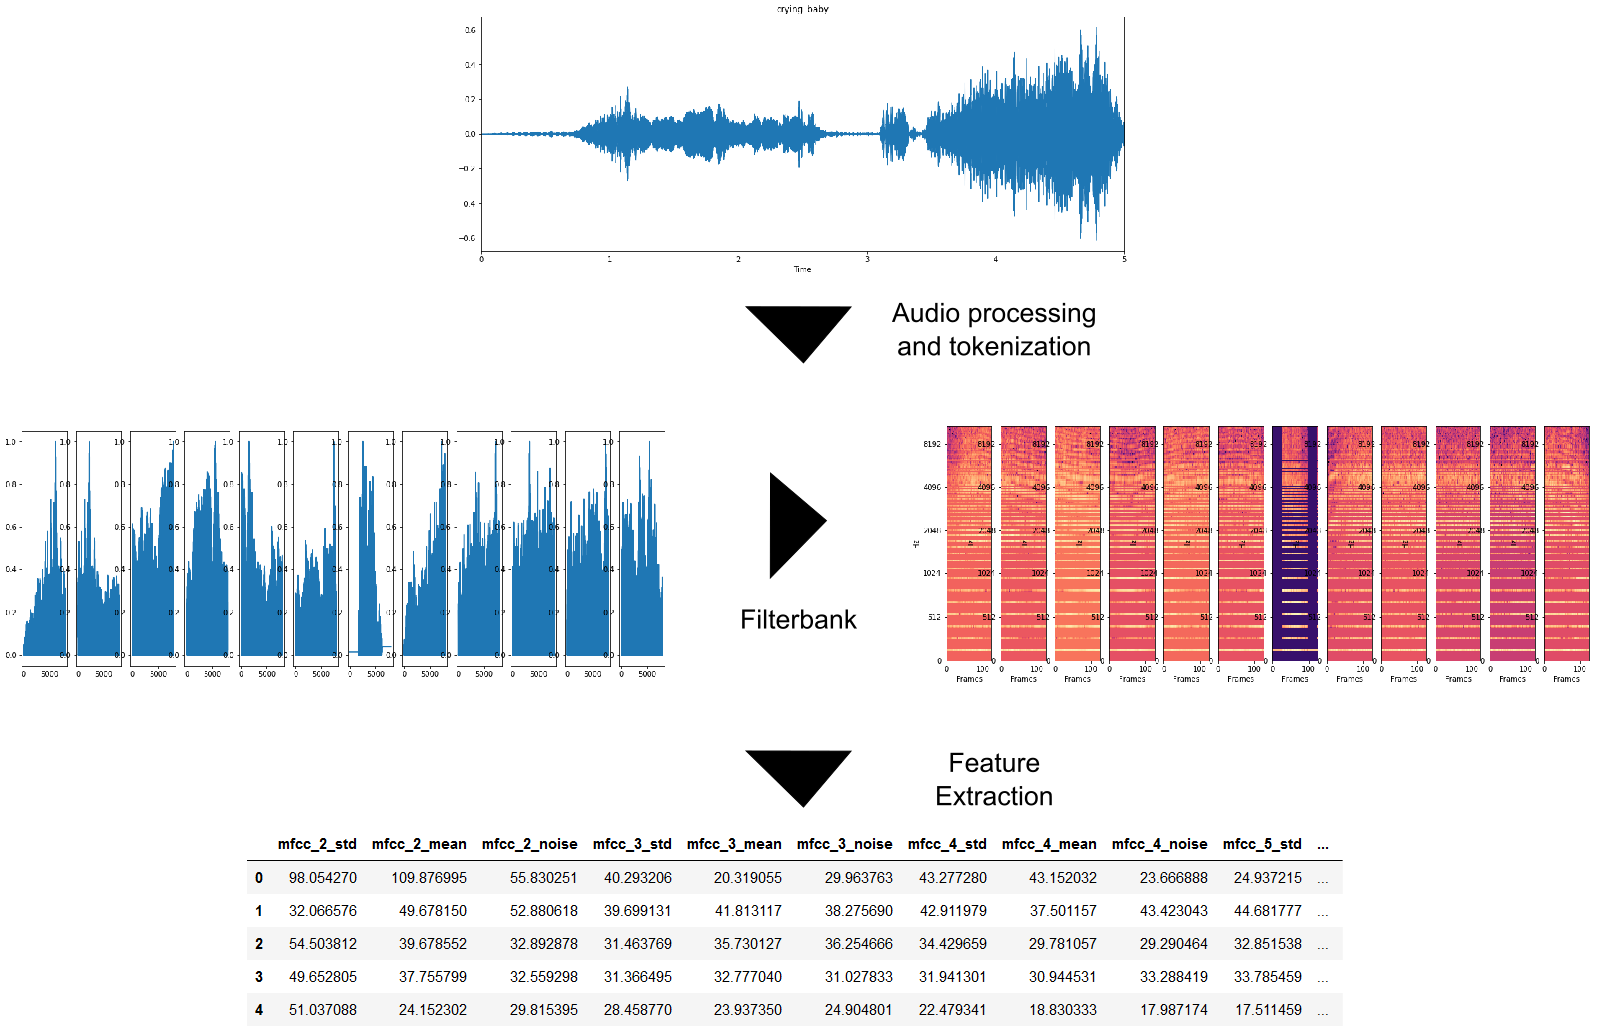
\includegraphics[width=0.7\textwidth]{figures/processing-pipeline.png}
    \caption{File processing pipeline.}
    \label{fig:my-label}
\end{figure*}

We present the set of features that we extract for facilitating audio retrieval
in~\cref{sec:representation::extraction}.
%
We next discuss how we transform these features and select a subset of the
transformed features that best suit the goals of system
in~\cref{sec:representation::transform}.

\subsubsection{Feature Extraction}
\label{sec:representation::extraction}

The feature set consists of both spectral and temporal features. 
%
Most of the chosen features are collected at a per-frame level (\ie, 
a matrix of values over the time window). 
%
All the features are extracted from short-time windows as described earlier.
%
The set of collected features include:

\squishitemize

\item \textit{Mel-frequency cepstral coefficients (MFCC)} capture the timbre
of the audio token. 
%
We use the first 13 coefficients calculated from a 40-channel filter bank.
%
The Mel-scale filter bank closely maps to the perceptual scale of pitches in
human hearing, as discussed in~\cref{sec:analyzer}. 

\item \textit{Spectral centroid} is the balancing point of the spectral power
distribution.

\item \textit{Spectral bandwidth} is the estimated bandwidth of the signal.

\item \textit{Spectral roll-off} captures the skew of the spectral shape. It
computes the frequency below which a certain amount of the spectral energy
resides.

\item \textit{Spectral flatness} The rationale behind this acoustic activity
detector is that the observed signal spectrum evinces more 'structure' when the
signal of interest is present compared to when it is absent.
%
This increase in the structure of the signal may be characterized by a 
reduction in the flatness of the magnitude spectrum of the signal\AJ{Cite?}.
%
Thus, setting an appropriate threshold on the flatness allows for detection of
the presence of the target signal.

\item \textit{Zero-crossing rate (ZCR)} is a measure of the number of zero
voltage crossing within an audio frame (obtained before half-wave
rectification).

\item \textit{Short-time average energy} is the sum of squared amplitudes 
within a frame representing the energy of a frame.

\item \textit{Root Mean Squared Energy} is the square root of the arithmetic
mean of the squares of the values, or the square of the function that defines the
continuous waveform.

\squishend

\PP{Matrix to Vector Transformation}
We apply statistical techniques to reduce this matrix to a vector. 
%
To reduce the representation to a vector while still retaining the data, we
collect a combination of statistics. 
%
We evaluate several combinations to determine the one that provides the most
information-dense feature vector. 
%
~\cref{tab:stats} summarizes the tested combinations of feature statistics 
and the number of derived descriptors.
%
\AJ{As many of these features are collected at a frame level statistics, found
in~\cref{tab:stats}, are computed over the entire window. --?}

\subsubsection{Feature Transformation}
\label{sec:representation::transform}

With all the collected and statistically-derived features, the vector contains
around 129 values.
%
Such a long vector presents an issue in training and evaluating classifiers
(\ie, the curse of dimensionality)\AJ{Cite?}.
%
We shrink the vector by applying feature selection and reduction techniques as 
a final preprocessing step.
%
Through experimentation, we found that the chi-square test and principal
component analysis to be the most effective techniques for feature selection and
reduction, respectively.

\PP{Feature Selection} 
%
We compute chi-squared stats between each non-negative feature and class.
% 
The chi-square test weeds out the features that are the most likely to be
independent of class by measuring the dependence between stochastic variables.
%
Thus, it selects the subset of features that are relevant for classification.

\PP{Feature Reduction}
%
We reduce the feature set using \textit{principal component analysis} (PCA).
%
PCA uses orthogonal transformations to convert a feature set of 
possibly correlated variables into a set of linearly uncorrelated variables
known as principal components. 
%
This technique allows us to provide a number of desired principal components,
thereby reducing the number of features in a controlled manner. 
%
However, the optimal number of principal components depends on the dataset 
and must be carefully chosen as the features may already be of sufficient
variance and dropping any will reduce the efficacy of the model. 
%
% This is an iterative technique with the first component being computed thus:
% \begin{equation}
%     \textbf{w}_{(1)} = \argmax_{||\textbf{w}||=1}{\sum_{i}(\textbf{x}_{(i)} \cdot \textbf{w})^2}
% \end{equation}
% %
% Here, \textbf{x} is a row vector of input data \textbf{X} and \textbf{w} is 
% the coefficient vector, constrained to be the unit vector. 
% %
% The subsequent components are computed by subtracting the first \textit{k} - 1
% principal components from \textbf{X} thus:
% \begin{equation}
%     \hat{\textbf{X}}_k = \textbf{X} - \sum_{s=1}^{k-1}{\textbf{X}\textbf{w}_{(s)}\textbf{w}_{(s)}^\textbf{T}}
% \end{equation}
% %
% and afterward finding a weight vector that extracts the maximum variance from
% the new data matrix:
% \begin{equation}
%     \textbf{w}_{(\textit{k})} = \argmax_{||\textbf{w}||=1}(||\hat{\textbf{X}}_{\textit{k}}\textbf{w}||^2)
% \end{equation}
% %
% It turns out in that the weight vectors computed using this iterative technique
% are eigenvectors of $ \textbf{X}^\textbf{T}\textbf{X} $.
%
We demonstrate that these feature transformation techniques effectively
shrink the feature vector in~\cref{sec:evaluation-encoding}.

\begin{figure}[t]
    \centering
    \includegraphics[width=0.45\textwidth]{example-image-a}
    \caption{Plot of feature reduced samples from music, animal, speech, and environmental sounds}
    \label{fig:top-dist}
\end{figure}

\section{Classification}

In this section, we present the architecture of the classification model in
\sys. 
%
We begin by making the case for a generalized model to enable performant and
accurate content-based audio retrieval in~\cref{sec:classification-case}.
%
We then present our two-level hierarchy of classifiers that is derived from 
machine hearing principles in~\cref{sec:classification-hierarchy}.
%
Lastly, we describe the methods used in \sys to serve as top-level and
bottom-level classifiers in~\cref{sec:classification-methods}.

\subsection{Case for a Generalized Classification Model}
\label{sec:classification-case}

In the audio domain, it is often desirable to train specialized models instead
of investigating general models. For example, performant models have been
developed for tasks like speech recognition or music genre recognition with
specific features chosen for the task \cite{Campbell1997,
tzanetakis-musical-2002}. However, these approaches are not applicable to the
general case of audio recognition. Here, we propose using and extending upon an
ecological taxonomy of sound for our recognition model in an effort to make it
generalizable to diverse databases.

Studies of human perception have long been of interest to ecologists, one in
particular created a taxonomy of environmental sound based on physical
properties and human perception. He hypothesized that in general listening
tasks, humans rely on seemingly complex stimuli and not a combination of the
senses as was previously thought which if true means that an agent can determine
sources through audio alone. Gaver posits that sound provides information of
audio items interacting in the environment and that these kinds of interactions
can be separated into several classes and sub-classes. This hypothesis of
hearing breaks the problem of decoding what we hear into much more generalizable
pieces that an agent can be trained on \cite{Gaver1993}. Although Gaver's
taxonomy only creates a taxonomy for interacting materials in the environment,
other researchers have similarly studied perception of animal vocalizations and
music.

Lewicki's work aids in gaining a better understanding of how animal sounds will
fit into a general sound taxonomy \cite{lewicki-efficient-2002}. It is noted by
Lewicki that environmental sounds are structurally different from animal
vocalizations in that animal vocalizations are longer, harmonic, and have a
narrow bandwidth while environmental sounds are transient, non-harmonic, and are
broadband. He hypothesizes that this has intentionally evolved to allow for
easier discrimination from environmental sounds when communicating. However,
Lewicki finds that human speech is structurally different from normal animal
vocalizations in that it contains a mix of harmonic and non-harmonic structures.
As such, in the taxonomy, speech and animal vocalizations are two separate
branches.

Both Gaver and Lewicki make a distinction between how we listen normally and how
we listen to music. As such, even though speech and interacting elements
technically make up music, how we listen to and classify musical sounds is
different. Thus, music in the taxonomy makes up its own branch in the hierarchy
indicating that once the agent determines a sound is music, it will begin
listening to it differently.

\subsection{Two-Level Hierarchy of Classifiers}
\label{sec:classification-hierarchy}

\begin{figure}[h!]
    \centering
    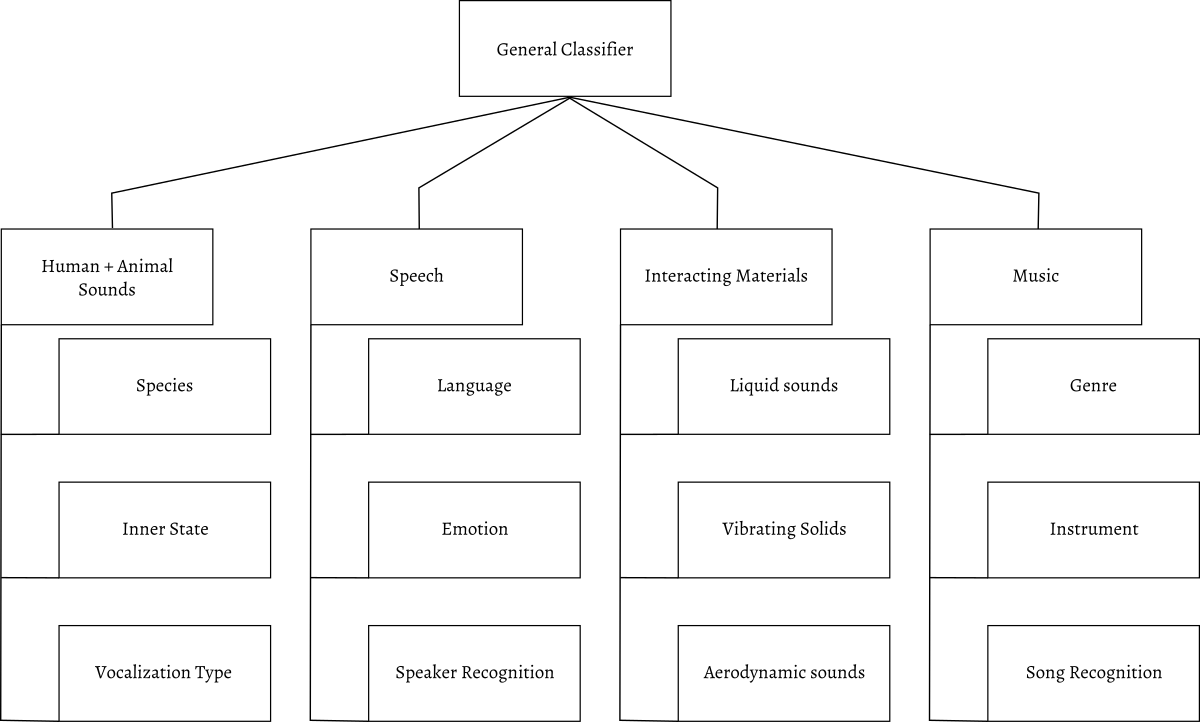
\includegraphics[width=0.49\textwidth]{figures/ensemble-overview.png}
    \caption{An overview of the proposed ensemble classifier.}
    \label{fig:classifier-hierarchy}
\end{figure}

Most classification tasks are what are called \textbf{flat classification}
meaning there is no hierarchy between the categories or if there is, it is
ignored. Our classification model instead uses the above taxonomy as a guide for \textbf{hierarchical classification} with a top-down approach. In a hierarchical model, multiple classifiers are trained on the same data. Unlike other ensemble methods though, this model trains each classifier with different goals \cite{chou-hierarchical-2003}. Here, we train a classifier per level of the tree. In evaluation, the algorithm follows a classification path, choosing a direction as each level is evaluated. This approach increases overall performance by breaking the classification task into smaller and less complex problems. Additionally, this approach allows us to throw out clearly irrelevant documents early, improving query runtime.

\subsubsection{Risks}
Error propagation is a major issue in this approach and if not managed can ruin the approach outright. Each classifier has some classification error inherent to it and as such a high error on higher level classifiers can seriously impede the efficacy of the system as a whole. We address this through use of probabilistic classifiers, enabling a measure of certainty, and how retrieval of documents is carried out.

Another consideration when working with a hierarchical classifier is whether the lowest level classes have enough examples to train a general model. If too few examples of a low-level class are in the database, the classifiers will begin to overfit. To mitigate this issue, another threshold policy is introduced. This time, the threshold is the minimum number of examples required to allow a classifier to be trained on a certain class. This results in instances of the model trained on a smaller database being less precise in their retrieval.

\subsection{Classification Methods}
\label{sec:classification-methods}

\begin{table}[t]
    \centering
    \begin{tabular}{ccc}
         & 250   & 2000  \\ \hline
    DNN  & 0.174 & 0.191 \\
    HDNN & 0.246 & 0.130
    \end{tabular}
    \caption{Classification results of a hierarchical DNN and a standard DNN trained on all 50 classes.}
    \label{tab:classifier}
\end{table}

%\begin{itemize}
    % \item Argue non-uniform classifier use
    % \item Filtering Classifiers
    % \item Deciding Classifiers
%\end{itemize}

Specific contexts of audio classification have long been an area of interest and thus certain audio sub-domains have been extensively studied for optimal classification techniques. It is unlikely that in human perception all different listening tasks are accomplished through the same process. Instead there are likely specialized systems that have evolved to best handle specific classification tasks. Using this intuition and the ability to do so through hierarchical classification, we pick and choose classifiers and representations that work best for each sub-domain. As this is a tree hierarchy, we have branch and leaf nodes that are comprised of their own classifier. Here, we term them \textit{Filtering} and \textit{Deciding} classifiers.

\subsubsection{Top-Level Classifiers}

\begin{table}[h]
    \begin{tabular}{c|cc}
        Classifier & Training & Prediction \\ \hline
        SVM & $O(n^2p+n^3)$ & $O(n_{sv}p)$ \\
        KNN & - & $O(np)$ \\
        RFC & $O(n^2\sqrt{p}n_{trees})$ & $O(pn_{trees})$
    \end{tabular}
\caption{Filtering classifiers and their properties.}
\label{tab:filt-class}
\end{table}

Filtering classifiers are the branch nodes of the hierarchy tree. They have this term as their main purpose is to filter the data and throw out unrelated documents such that lower filter and deciding classifiers can execute more quickly. In our experiments, it was found to be desirable for these classifiers to be both lightweight and have uncertainty associated with it. As such, probabilistic classifiers are used in the filtering classifiers. 

Probabilistic classifiers are key to mitigating the issue of error propagation in the hierarchical model. While standard classifiers emulate a function of the form $y=f(x)$ with a single result \textit{y} for each input \textit{y}, a probabilistic classifier instead emulates conditional distributions of the form $P(y|x)$. We are able to use the resulting probabilities given by a classifier to determine its confidence in the prediction made. We use this confidence to allow normally misclassified results to still be considered in later steps. This is done by introducing a threshold $\gamma$ that must be reached to proceed. If the threshold is too low, we lose the performance efficacy of the hierarchical structure. On the other hand, if the threshold is too high then false negatives will ensure some documents with harder to classify instances of a class will never be retrieved.

In this implementation, the following lightweight and probabilistic classifiers were experimented with:
\\
\\
\textbf{Support Vector Machines} are a supervised learning model used for classification that partitions the data by finding the most optimal linear hyper-plane that separates all dimensions of the feature set optimally. Although SVMs inherently separate the data by some linear relationship (decision boundary), non-linear classification can be done by the kernel trick. The kernel trick is the method of mapping the inputs into different feature spaces in which the data is linearly separable. To allow for probabilistic estimation, the SVM is computed with soft-margins. The soft-margins provide a decision boundary with in-built uncertainty through a gradient of certainty that becomes greater as samples are picked further from the boundary. The boundary is calculated by minimizing the the hinge loss function over all samples. This is calculated by

\begin{equation}
    \Big[ \frac{1}{n}\sum^n_{i=1}\max(0,1-y_i(\vec{\omega} \cdot \vec{x_i} - b))\Big] + \lambda ||\vec{\omega}||^2
\end{equation}
\\
where $\omega$ is the normal vector to the hyper-plane, $y_i$ is the target, $\vec{x_i}$ is the features at i, and $\lambda$ determines the margin size and whether $\vec{x_i}$ is on the correct side of the decision boundary. For small values of $\lambda$, the soft-margin SVM will perform similarly to the hard-margin.
\\
\\
\textbf{K-Nearest Neighbors} is a classification method that uses the plurality vote of its neighbor samples by some heuristic of distance to determine its belonging to a class. KNN is known as a \textit{lazy learning} method, meaning the classifier defers its computation until classification evaluation. As such, all points are retained in the model. Any custom heuristic for distance can be used but the most common is Euclidean distance or Manhattan Distance. One of the more challenging parts of this classification approach is the tuning of the neighbor number hyper-parameter as at k=1 the class is determined by the first closest neighbor and at k=n the class is whatever the most numerous of the classes is present. To use this classifier in a probabilistic case, the number of matching neighbors and the distances can be used for determination. Probability is computed such that the radial area surrounding the k neighbors creates a probability distribution. \cite{cheng-evaluating-2009}
\\
\\
\textbf{Probabilistic Random Forests} are a supervised ensemble classification learning method. This method uses a collection of decision tree classifiers and at evaluation time provides the mode of the classification prediction. This method attempts to correct for decision trees tendency to overfit the training set. Specifically, deep trees more often tend to overfit, have low bias, and very high variance. Thus, by training many trees on multiple parts of the data, it is expected that variance will be reduced with only a small increase in bias. To train a random forest, the bagging algorithm is employed. This algorithm takes a training set and selects a random sample with replacement to fit a tree to. The bagging approach decreases the model variance, which as mentioned before is a problem in decision trees, and only slightly increases the bias. Evaluation of the model is straightforward as it is either an average of the data in the regression case or is majority vote in classification. To provide probability to the random forest classifier, the choice between two paths is treated as a probability density function (pdf) and both branches are evaluated if it meets some criterion for acceptable probability bounds \cite{reis-probabilistic-2018}. This approach modifies the \textit{Gini impurity} function

\begin{equation}
    G_n \xrightarrow{}    \bar{G_n} = 1 - \sum_{j=1 \dotsc k} \bar{P}_{n,A_j}
\end{equation}

% \subsubsection{Annotation Normalization} Annotation normalization is carried
% out on subsets of both the ESC-50 and AudioSet database. Performance is
% measured in terms of execution time, efficiency, and overall annotation
% reduction. The normalization performance is measured against human performance
% and Hsu's normalization results \cite{Hsu2008}. As ESC-50 already has its
% annotations manually normalized, the normalization experiments demonstrate if
% the techniques go too far and overgeneralize. Additionally, it provides a
% clean test-bed for hypernyms to be evaluated. For hypernym sets, we hope to
% have sets that as much as possible attempt to distribute the database across
% them. AudioSet presents a much greater challenge for the low level
% normalization task. These experiments give insight into how the technique
% works at scale and what bottlenecks exist.

\subsubsection{Bottom-Level Classifiers}

\begin{table}[h]
    \begin{tabular}{c|cc}
        Classifier & Training & Prediction \\ \hline
        DNN & $O(n^4)$ & $O(n^5)$ \\
        RNN & $O(n^4)$ & $O(n^5)$ \\
        GMM & $NP$ & $a$
    \end{tabular}
    \caption{Decision classifiers and their properties.}
    \label{tab:dec-class}
\end{table}
Deciding classifiers are those found on the leaf nodes of the hierarchy tree. These classifiers have the purpose of making some determination on the remaining data and as such are able to be much more definitive with their result. In particular, this means the models at these leaf nodes are able to be more complex and take longer per sample to execute as ideally much of the database has been ruled out already. We do however, retain probabilistic classification because it serves as a heuristic for ranking the retrieved documents.
\\
\\
\textbf{Deep Neural Networks} are a method of supervised classification that forms a feed-forward graph of connected neurons that only activate if some threshold is met. A neural network is meant to model a collection of neurons in the human brain with them only activating if sufficiently excited. Even though this model falls short of actually modeling neurons, it performs well in many applications. Network neurons are organized into layers that form a row of neurons that is normally fully connected to the previous row or, in the base case, the inputs. A network can be as simple as a single layer, but in most applications a large number of layers and neurons are required. Unfortunately, the algorithm that trains these networks is computationally expensive and on single thread computers can take hours to converge. However, the algorithm is embarrassingly parallel and thus can be much more efficiently performed on GPU or TPU hardware. This allows for networks to be much larger and more complex without needing to sacrifice training time, these networks are known as Deep Neural Networks (DNN). To determine the probability of each class predicted, the final layer is evaluated with the softmax function as in probability theory it is used to represent a categorical distribution.
\\
\\
\textbf{Recurrent Neural Networks} are an extension of neural network with the major difference that they have a temporal component. To account for this new component, the backpropagation algorithm is modified to the backpropagation through time algorithm in which time is expresed by an ordered series of calculations linking one time step to the next allowing backpropagation to proceed as usual. The process of carrying memory forward can be described as

\begin{equation}
    h_t=\phi(Wx_t+Uh_{t-1})
\end{equation}
\\
with $h_t$ the hidden state at time t, $x_t$ the input at time t, $W$ the weight matrix, and $U$ the transition matrix. Although there is more information from the past, these neural networks also share the vanishing gradient issue deep neural networks have. Long Short-Term Memory units (LSTMs) were introduced in an attempt to solve the vanishing gradient problem. LSTMs contain information in a gated cell that can be written to or read from and only allows these operations if some analog value passes a threshold. By gating with a differential value, the backpropagation algorithm can iteratively determine when it is best to recall, write, or forget the stored information. This allows the network to use data from layers more than one layer behind it.
\\
\\
\textbf{Gaussian Mixture Model} is a probabilistic model assuming the data are generated by a number of Gaussian distributions with unknown parameters. GMMs are able to be trained either in an unsupervised or supervised manner, in this approach we use the supervised approach. The model is trained using the expectation-maximization algorithm which determines the component weights, means, and variances. Although this approach has seen success on many audio applications in the past, training complexity is high and thus training on large datasets is time intensive. This model is naturally probabilistic and as such no extra steps need to be taken for probability estimation.
\\

\section{Retrieval}
\begin{itemize}
    \item 
\end{itemize}
\section{Evaluation}

\subsection{Training Datasets}
\begin{figure}
    \centering
    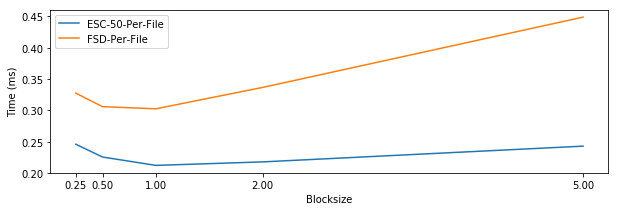
\includegraphics[width=0.45\textwidth]{figures/dataset-load-time.png}
    \caption{Caption}
    \label{fig:load-time}
\end{figure}

The datasets chosen for training are ideally clean, uniform and have about an equal number of each class instance. 

The system depends on the ability of the machine learning agent to be able to
match between acoustic features and the text queries. Its performance depends on
both the size of the database and the specificity of the query. To examine
performance across environments, we choose a clean and a dirty database: ESC-50
\cite{Piczak2015} and Freesound.

\\
\textbf{ESC-50} This clean database is made available on GitHub for environmental sound
classification. It is maintained such that the tag vocabulary is fixed and each
audio document attempts to only contains a single object in it. Each document is
5 seconds long and audio quality in terms of samplerate and recording noise is
normalized across the database. This makes for a very clean database with little
noise in both audio and annotation. It has 50 semantic classes with 40 examples
per class arranged into 5 major categories. However, the major categories do not
match the Gaver taxonomy and so were manually separated as in Table
~\ref{tab:relabel}. The database's sound documents come from the Freesound
project with the author providing uniform tags and normalizing the audio
manually \cite{Font2013}.

\\
\textbf{Freesound} The Freesound database is made up entirely of user-submitted and tagged audio documents. This is used to test the efficacy of the method on a real-world unstructured database. The documents in the database are in a variety of audio formats and lengths. Additionally, a portion of the documents contain multiple audio objects that overlap.

\subsection{Window Size}
Choosing the size of the window determines the granularity of the feature vector as each window's feature matrix is reduced into a vector for training. If the window is too large we obtain a single feature vector, but it is likely too generic to be useful in classification. On the other hand, a window that is too small will increase the time required to complete preprocessing, training, and evaluation steps and increase the size of the feature table. To determine the optimal window size, we evaluated five window sizes with each high-level classifier. The optimal window size is the one that balances training time, evaluation time, and classification accuracy.

\subsubsection{Preprocessing}


\subsubsection{Encoding Results}
\label{sec:evaluation-encoding}

\begin{figure}[h]
    \centering
    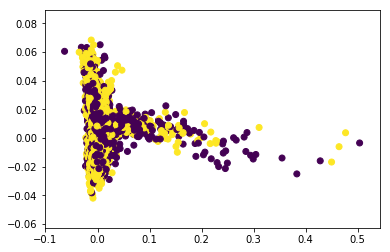
\includegraphics[width=0.45\textwidth]{figures/pca-cluster-hl.png}
    \caption{2D clustering of features using PCA.}
    \label{fig:pcahl}
\end{figure}

\begin{table}[t]
    \centering
    \begin{tabular}{c|cc}
    \textbf{Window} & \textbf{Read} & \textbf{Process} \\ \hline
    250              & 7840           & 37318                    \\
    2000             & 2413           & 4831                   
    \end{tabular}
    \caption{The average read and processing time in ms for 400 documents.}
    \label{tab:base-time}
\end{table}

\subsubsection{Training Evaluation}

\begin{figure}
    \centering
    \includegraphics[width=0.45\textwidth]{example-image-a}
    \caption{Comparative training time between PAMIR, WARP, and ECHO (what we're calling this system?)}
    \label{fig:my-label}
\end{figure}

\begin{figure}
    \centering
    \includegraphics[width=0.45\textwidth]{example-image-a}
    \caption{Plot of training iterations needed before getting diminishing returns (comparative between classifiers)}
    \label{fig:learning-curve}
\end{figure}

\subsubsection{Representation Experiments}

\begin{table}[]
    \begin{tabular}{llllll}
    Classifier/Window       & 250 ms & 500 ms & 1 s   & 2 s  & 5 s   \\
    Deep Neural Nets        & 0.628  & 0.653  & 0.656 &      &       \\
    Random Forest           & 0.66   & 0.68   & 0.68  & 0.64 & 0.69  \\
    K-Nearest Neighbors     & 0.61   & 0.62   & 0.62  & 0.65 & 0.64 \\
    Support Vector Machine  & 0.62   & 0.64   & 0.62  & 0.62 & 0.67   
    \end{tabular}
\end{table}

Classifier performance at different window sizes and features (remember, have run wavenet)

\begin{figure}[h]
    \centering
    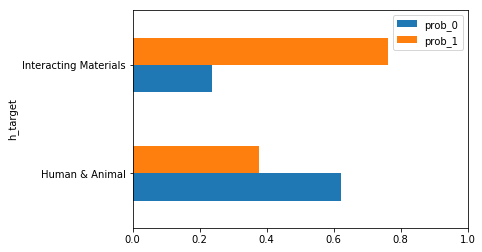
\includegraphics[width=0.45\textwidth]{figures/knn-prob-plot.png}
    \caption{Plot of average probabilities for each class of the misclassified documents at the top level.}
    \label{fig:a}
\end{figure}

\subsubsection{High-Level Classification}

\begin{figure}
    \centering
    \subfloat[SVM]{{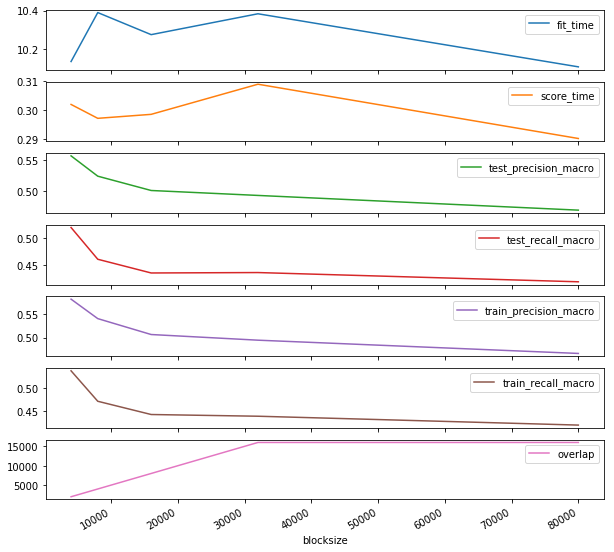
\includegraphics[width=0.25\textwidth]{figures/FSD-SVM.png}\label{fig:fsd-svm}}}
    \subfloat[KNN]{{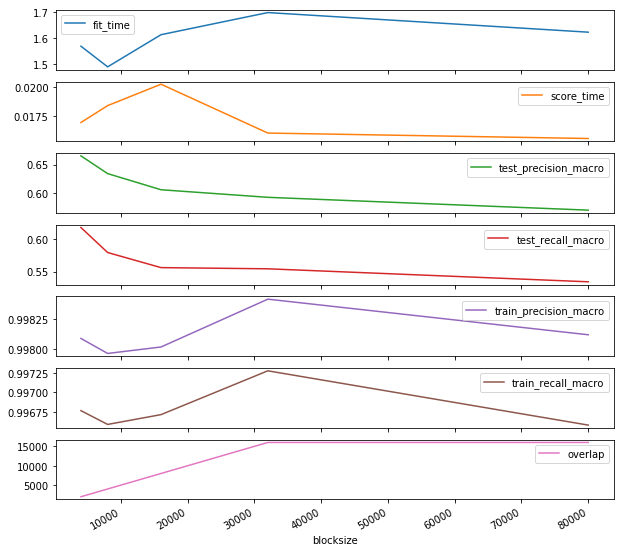
\includegraphics[width=0.25\textwidth]{figures/FSD-KNN.png}\label{fig:fsd-knn}}}
    \hfill
    \subfloat[RFC]{{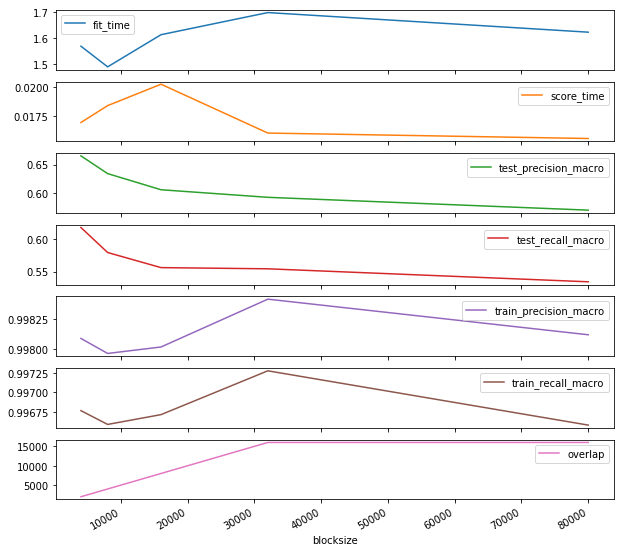
\includegraphics[width=0.25\textwidth]{figures/FSD-RFC.png}\label{fig:fsd-rfc}}}
    \caption{Training and testing statistics of high level classifiers on the FreeSound Database.}
\end{figure}

\begin{figure}
    \centering
    \subfloat[SVM]{{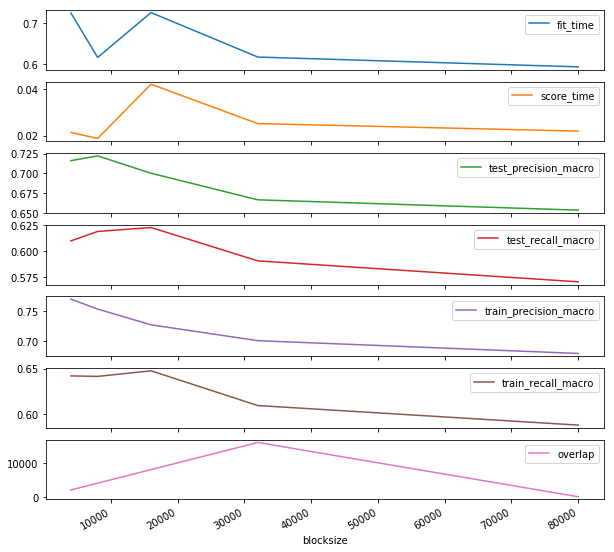
\includegraphics[width=0.25\textwidth]{figures/ESC-50-SVM.png}\label{fig:esc-50-svm}}}
    \subfloat[KNN]{{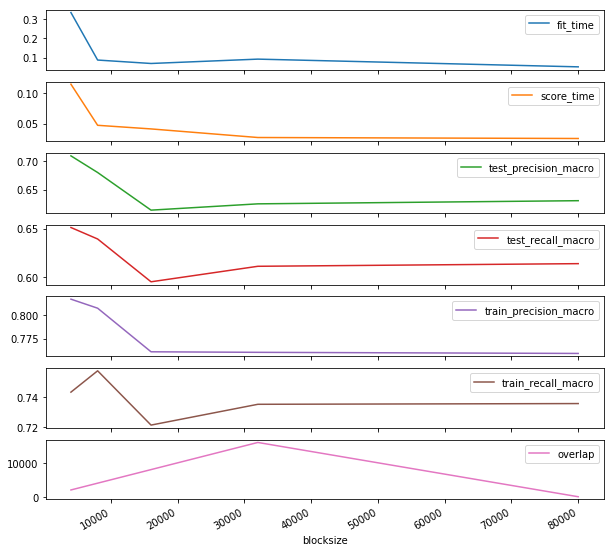
\includegraphics[width=0.25\textwidth]{figures/ESC-50-KNN.png}\label{fig:esc-50-knn}}}
    \hfill
    \subfloat[RFC]{{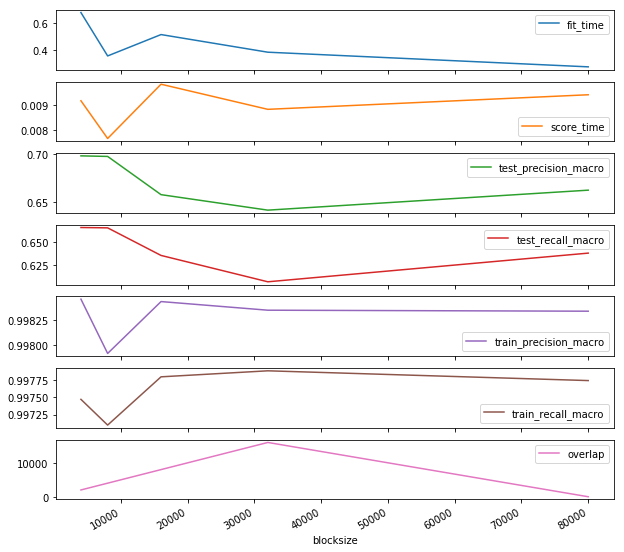
\includegraphics[width=0.25\textwidth]{figures/ESC-50-RFC.png}\label{fig:esc-50-rfc}}}
    \caption{Training and testing statistics of high level classifiers on the ESC-50 Database.}
\end{figure}

\subsubsection{Low-level Classification}

\begin{figure}
    \centering
    \subfloat[SVM]{{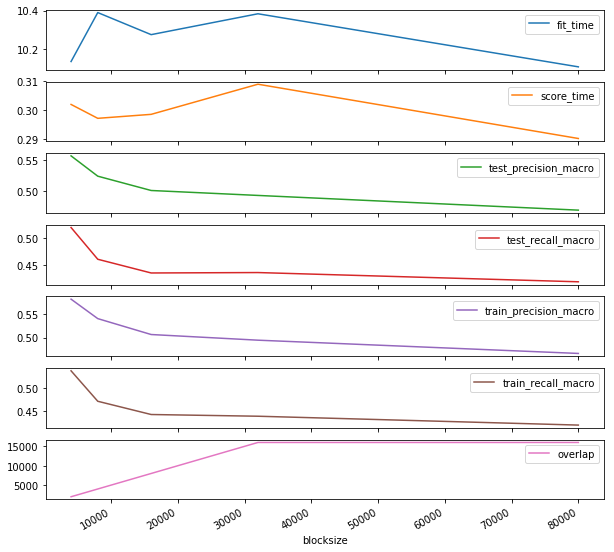
\includegraphics[width=0.25\textwidth]{figures/FSD-SVM.png}\label{fig:fsd-svm}}}
    \subfloat[KNN]{{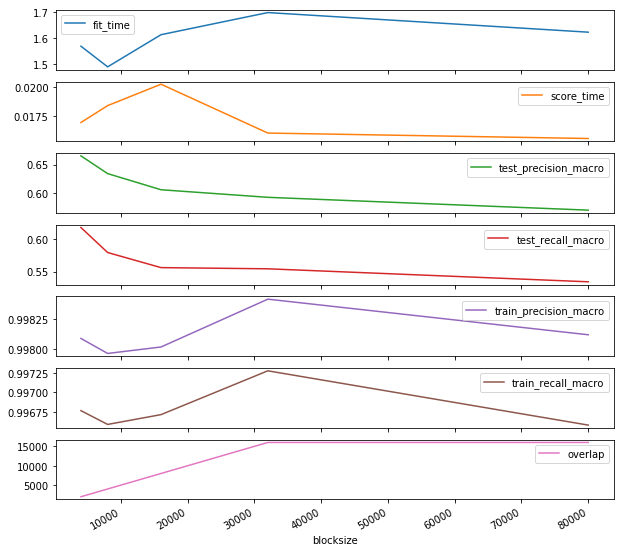
\includegraphics[width=0.25\textwidth]{figures/FSD-KNN.png}\label{fig:fsd-knn}}}
    \hfill
    \subfloat[RFC]{{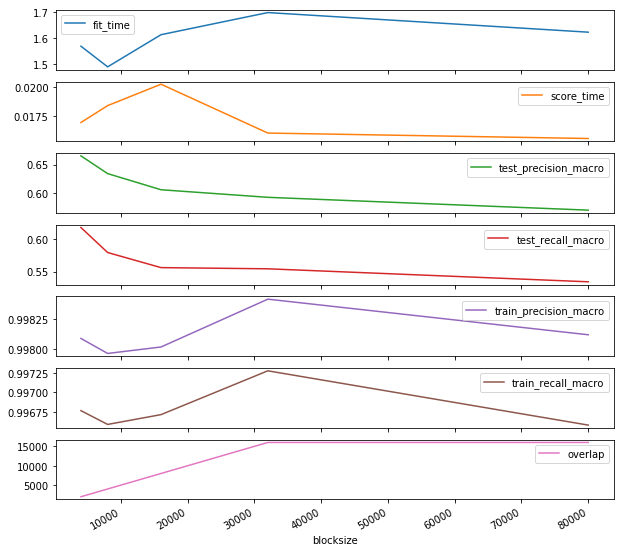
\includegraphics[width=0.25\textwidth]{figures/FSD-RFC.png}\label{fig:fsd-rfc}}}
    \caption{Training and testing statistics of high level classifiers on the FreeSound Database.}
\end{figure}

\begin{figure}
    \centering
    \subfloat[SVM]{{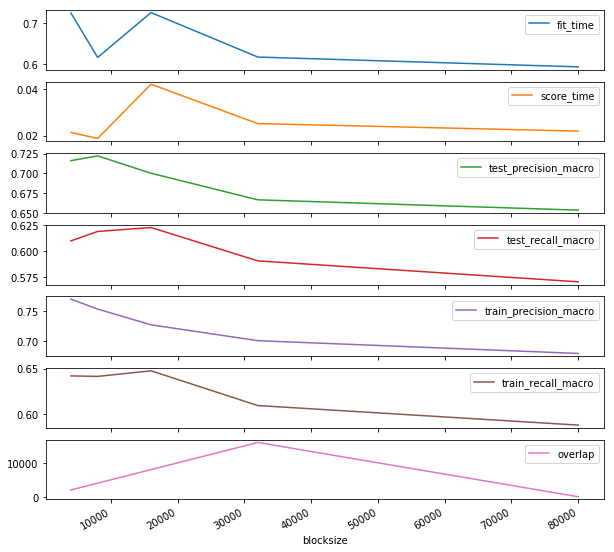
\includegraphics[width=0.25\textwidth]{figures/ESC-50-SVM.png}\label{fig:esc-50-svm}}}
    \subfloat[KNN]{{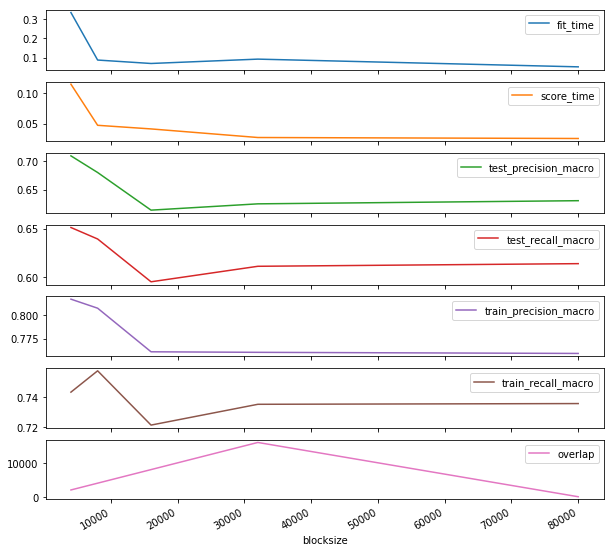
\includegraphics[width=0.25\textwidth]{figures/ESC-50-KNN.png}\label{fig:esc-50-knn}}}
    \hfill
    \subfloat[RFC]{{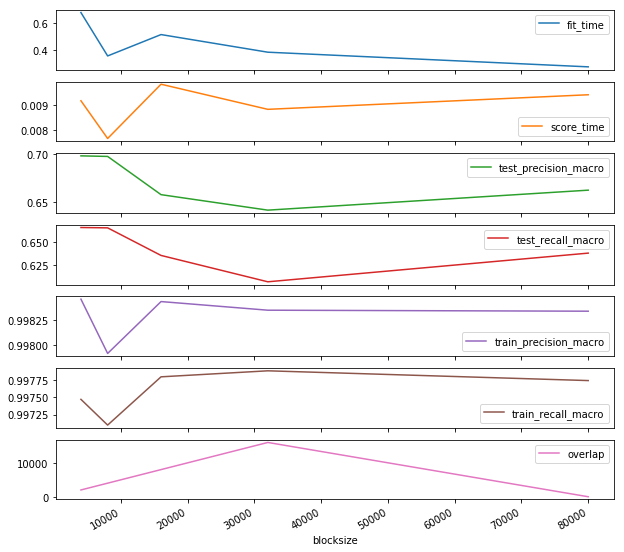
\includegraphics[width=0.25\textwidth]{figures/ESC-50-RFC.png}\label{fig:esc-50-rfc}}}
    \caption{Training and testing statistics of high level classifiers on the ESC-50 Database.}
\end{figure}

\subsubsection{Full Classification Performance}

Cross-validated performance of each subclassifier and performance of hierarchical

\subsubsection{Retrieval Performance (Time + Accuracy)}


\section{Conclusion}
The approach here shows promise, especially in the context of a retrieval
system. Using human perception as a model is an approach that had been pursued
in machine vision with success and it is only logical to do the same for machine
listening. By understanding the mechanisms by which we convert auditory signals
to brain signals, we can understand how the audio needs to be encoded for use in
machine hearing. One of the aspects of audio we have yet to optimally integrate
are temporal features which are of utmost importance in audio signals.

To this end, several representations were attempted in this work. The first was
just basic feature extraction from spectral representations of the audio using
librosa. Librosa allowed for many spectral and temporal features to be taken
from the signal though it is a slow process and may still not provide a good
feature set. To better emulate human perception, auto-encoders were attempted
next. The thought was that a neural network will be able to find latent
variables that are of better use than those extracted from usual means. However,
it was found that this approach did not bear out and hardly effected
performance.

Experiments were run comparing this approach to two off-the-shelf classifiers on
each layer of the hierarchy. The SVM classifier consistently under-performed and
will likely be removed from subsequent evaluations. A Random Forest Classifier
was consistently about equal to the neural networks it was evaluated against but
in nearly every case, the network was able to beat its precision score.

Overall, this study provided insights into the complexity of autonomous audio
analysis and the challenges that are still facing the field. of these
challenges, it seems that representation is the most pressing. It appears though
that the current direction of studying human perception mechanisms and emulating
them will prove optimal.


\input{related-works.tex}
\section{Future Work}

The hierarchical approach in its current iteration only provides minimal
improvement over standard DNNs. However, the lessons learned here provide a
basis on which to build out a more performant system. First, representation will
be revisited and recurrent neural networks will be employed to aid in creating a
new representation that considers audio's temporal nature. Second, more specific
probabilistic neural networks will be investigated for integration into the
\textit{Animal Voices} and \textit{Interacting Materials} classification tasks.
Finally, a querying front-end will be developed for this and will be used for
querying of the AudioSet database.

%% ==================================================================
%% BIBLIOGRAPHY
%% ==================================================================
\newpage

\bibliographystyle{abbrv}
\small
\raggedright
\bibliography{references}

\end{document}
